\documentclass[notheorems, handout]{beamer}

\usetheme{Warsaw}
\setbeamertemplate{page number in head/foot}[totalframenumber]
\setbeamertemplate{headline}{}
\setbeamertemplate{navigation symbols}{}
\usefonttheme[onlymath]{serif}

\usepackage[utf8]{inputenc}
\usepackage[T2A]{fontenc}
\usepackage[russian]{babel}
\usepackage{graphicx,subcaption,ragged2e}
\usepackage{tikz}
\usepackage{bm}
\usepackage{physics}
\usepackage{amsmath,amsfonts,amssymb}
\usepackage{mathtools}

\newtheorem{theorem}{Теорема}

\title[Нейронные сети и Deep Learning]{Нейронные сети (NN) \\ с элементами Deep Learning}

\institute[Санкт-Петербургский Государственный Университет]{%
  \small
  Санкт-Петербургский государственный университет\\
  Кафедра статистического моделирования
}
\date{18 октября 2025}
\newcommand{\vect}[1]{\mathbf{#1}}
\newcommand{\matr}[1]{\boldsymbol{#1}}


\begin{document}

\begin{frame}
    \titlepage
\end{frame}
\begin{frame}
    \frametitle{Что такое нейронные сети?}
    \begin{itemize}
        \item Нейронные сети --- это семейство моделей машинного обучения, которые стали доминирующим подходом во многих областях с 2012 года.
        \item Идея была предложена еще в 1970-х, но технические возможности для обучения больших сетей появились только в начале 2010-х.
        \item Совокупность нейросетевых подходов называется \textbf{глубинным обучением} (Deep Learning).
    \end{itemize}
\end{frame}

\begin{frame}
    \frametitle{Две ключевые идеи Deep Learning}
    \begin{columns}[c]
        \column{.5\textwidth}
        \textbf{End-to-end обучение}
        \begin{itemize}
            \item<2-> Переход от сложных пайплайнов, где каждая часть решает свою подзадачу, к обучению всей системы как единого целого.
            \item<3-> Например, вся модель от сырых данных до конечного ответа обучается совместно.
        \end{itemize}

        \column{.5\textwidth}
        \textbf{Обучение представлений (Representation Learning)}
        \begin{itemize}
            \item<2-> Автоматическое создание информативных признаков из данных, часто неразмеченных.
            \item<3-> Это позволяет отказаться от ручного конструирования признаков экспертами.
        \end{itemize}
    \end{columns}
\end{frame}

\begin{frame}
    \frametitle{Полносвязные нейросети}
    \begin{itemize}
        \item Самая простая архитектура нейронных сетей.
        \item Состоит из слоев, в каждом из которых есть \textbf{нейроны}.
        \item Нейроны одного слоя соединены со всеми нейронами следующего слоя.
    \end{itemize}
    \begin{figure}
        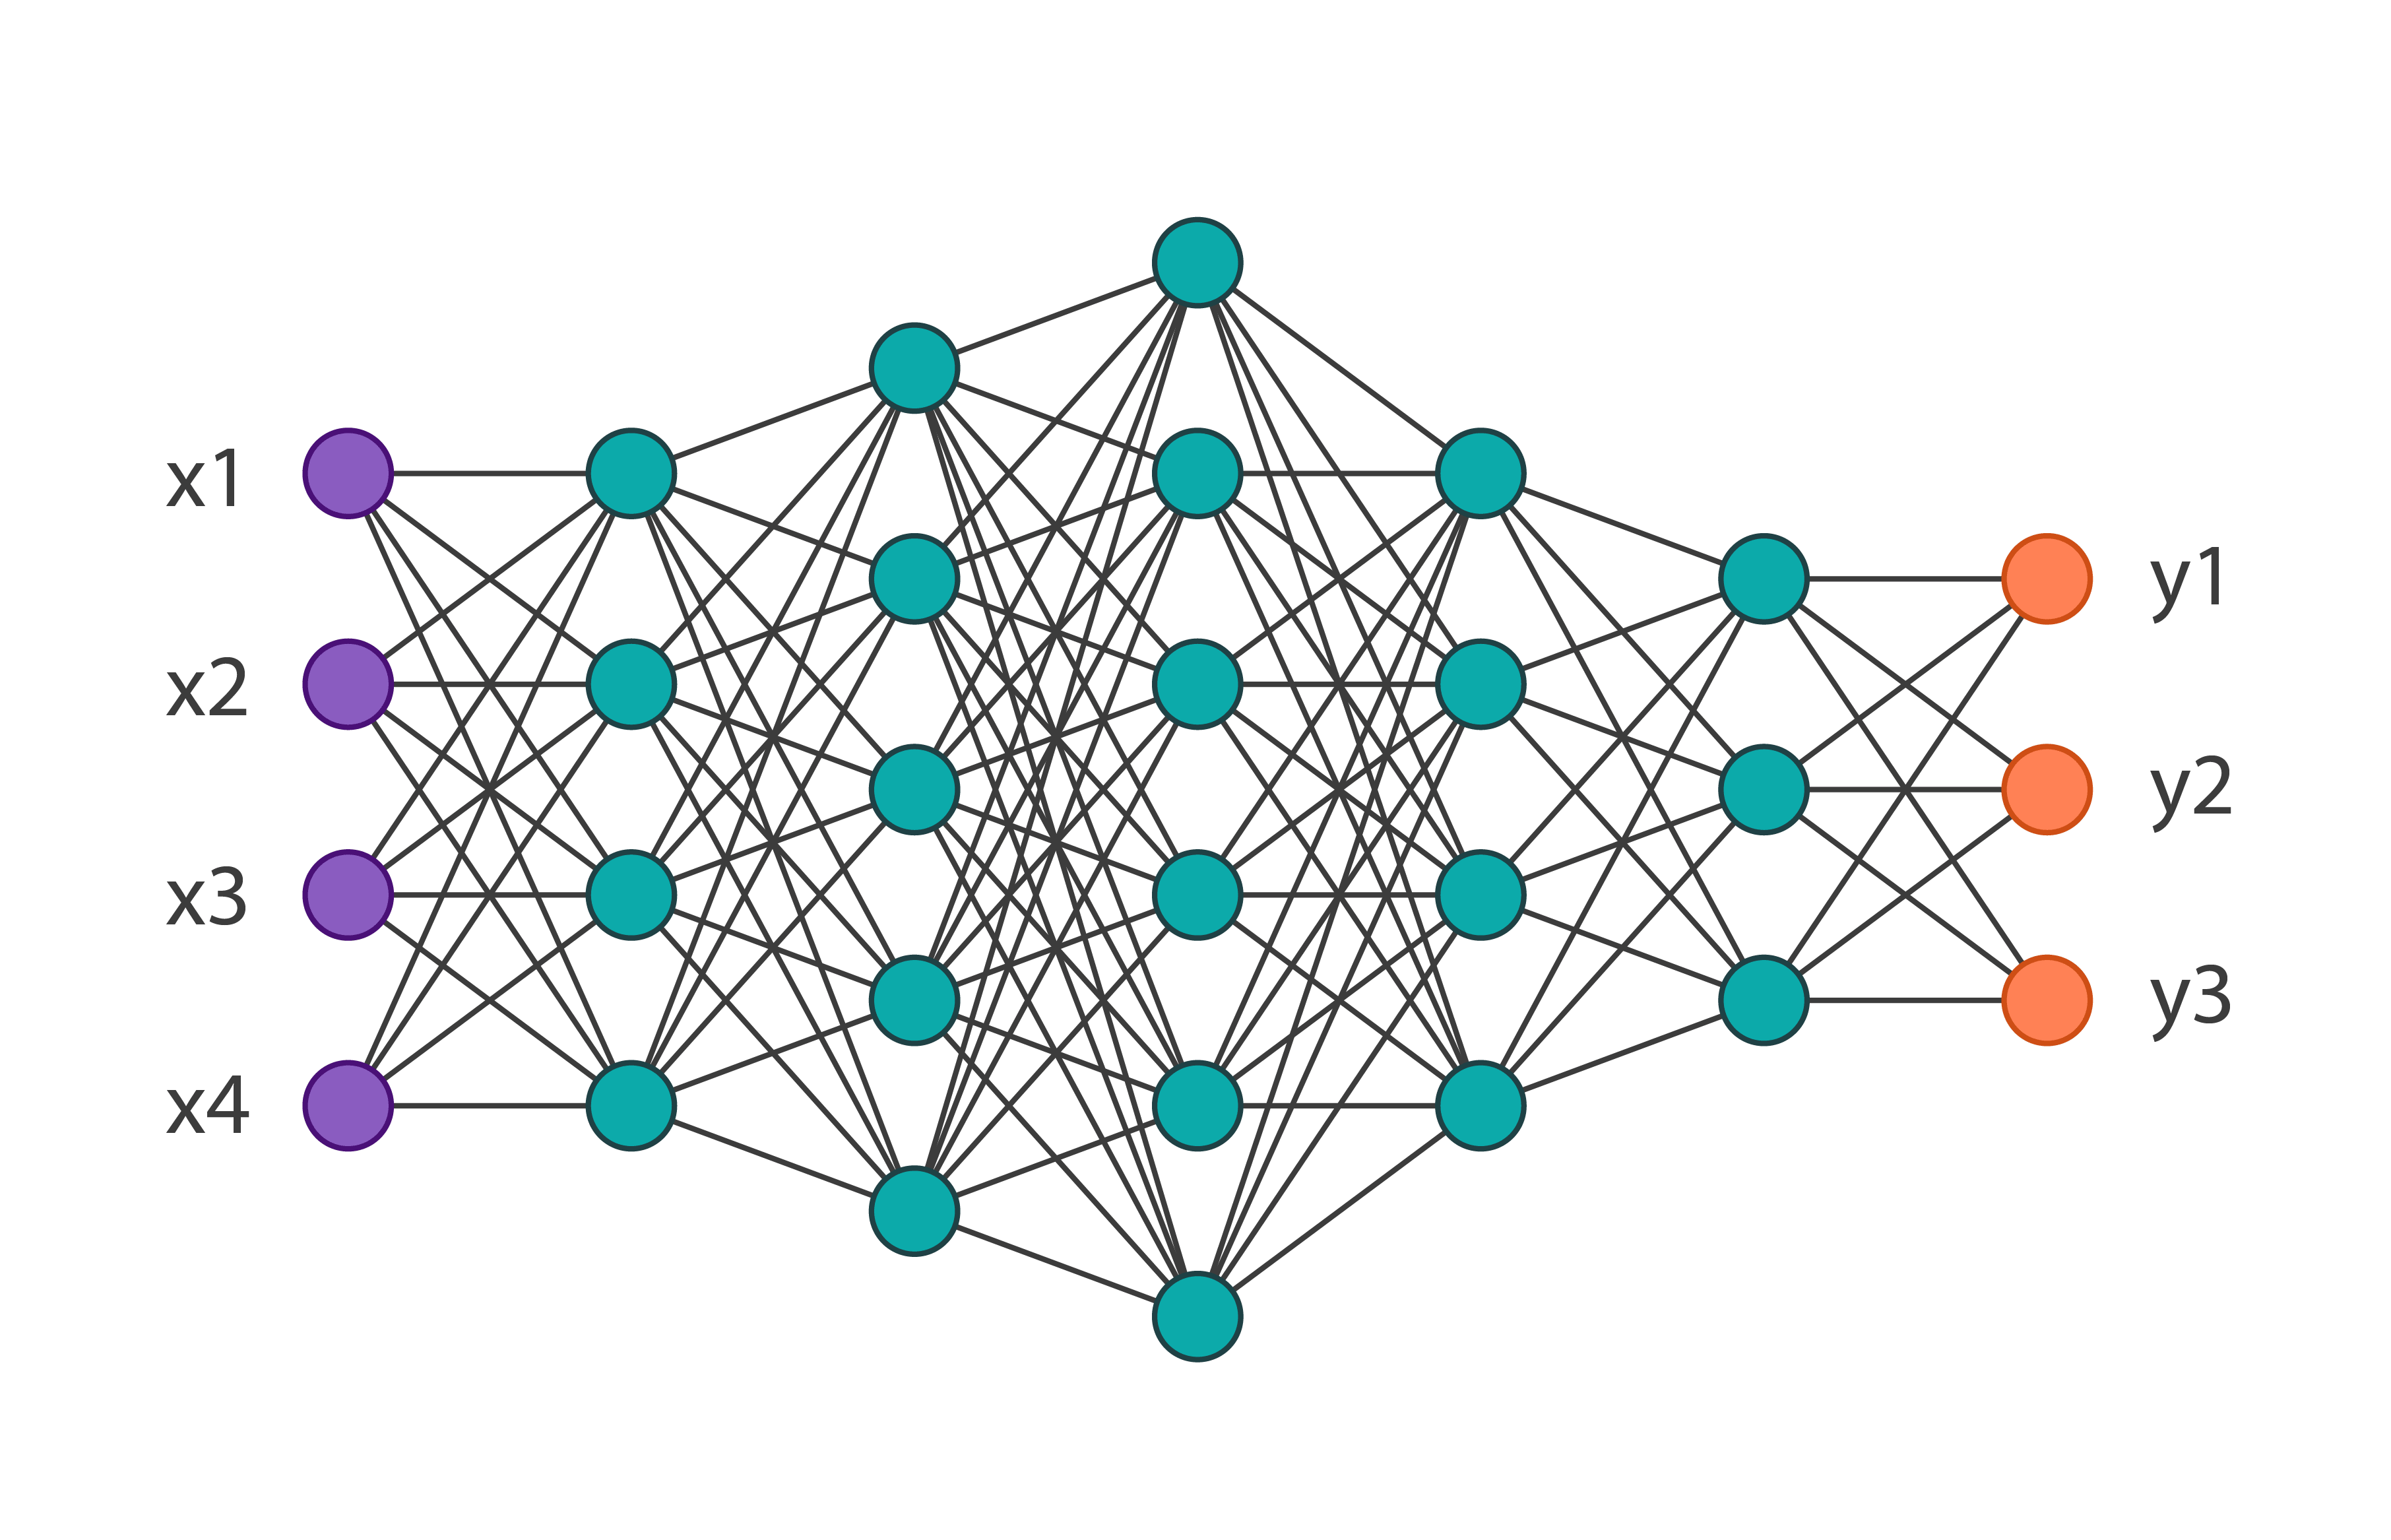
\includegraphics[width=0.7\textwidth]{img/fnn.png}
        \caption{Пример структуры полносвязной нейронной сети.}
    \end{figure}
\end{frame}

\begin{frame}
    \frametitle{Из чего состоит нейрон?}
    \begin{itemize}
        \item \textbf{Входы ($x_i$)}: значения, поступающие от предыдущего слоя.
        \item \textbf{Веса ($w_i$)}: параметры, которые показывают важность каждого входа.
        \item \textbf{Смещение ($b$)}: дополнительный обучаемый параметр.
        \item \textbf{Сумматор}: вычисляет взвешенную сумму входов: $z = \sum_{i} w_i x_i + b$.
        \item \textbf{Функция активации ($f(z)$)}: нелинейная функция, которая определяет выходной сигнал нейрона. Примеры: Sigmoid, ReLU.
    \end{itemize}
\end{frame}

\section{Отдельный нейрон и слой}

\begin{frame}
    \frametitle{Что такое нейрон? Математическая модель}
        Нейрон --- это базовая вычислительная единица сети. Он выполняет два последовательных действия:
  \begin{columns}[T]
        \column{.55\textwidth}

        \begin{enumerate}
            \item \textbf{Аффинное преобразование}: вычисляет взвешенную сумму своих входов ($x_i$) с весами ($w_i$) и добавляет смещение ($b$). Это называется \textbf{логитом}.
            \item \textbf{Нелинейное преобразование}: применяет к результату \textbf{функцию активации} $f(z)$.
        \end{enumerate}
        \column{.45\textwidth}
        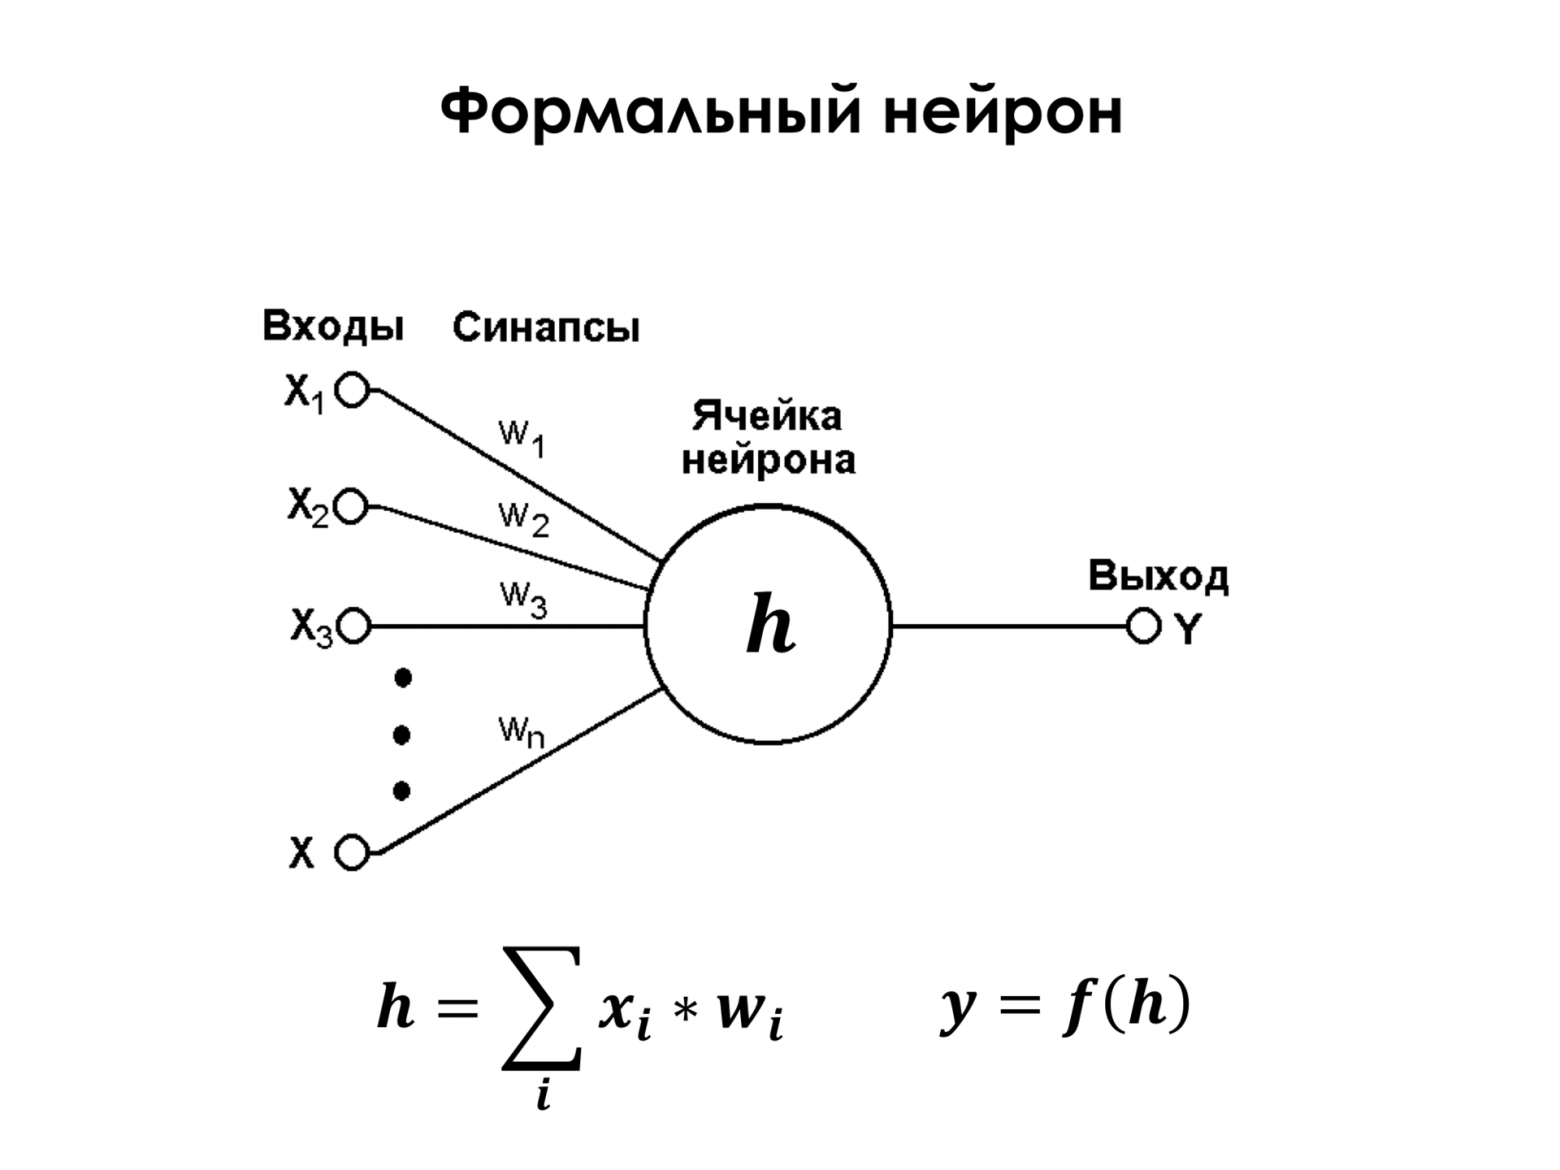
\includegraphics[width=1.2\textwidth]{img/neuron.png}
    \end{columns}
    \vspace{1em}
    \begin{block}
    \centering
    Логит: $z = w_1 x_1 + w_2 x_2 + \dots + w_n x_n + b = \sum_{i=1}^{n} w_i x_i + b$ \\
    Выход нейрона: $a = f(z) = f\left(\sum_{i=1}^{n} w_i x_i + b\right)$
    \end{block}
\end{frame}

\begin{frame}
    \frametitle{Векторная форма для нейрона}
    Для удобства и эффективности вычислений операции записываются в векторной форме.
    \begin{itemize}
        \item Входные данные: вектор $\mathbf{x} = [x_1, x_2, \dots, x_n]^T$
        \item Веса: вектор $\mathbf{w} = [w_1, w_2, \dots, w_n]^T$
        \item Смещение: скаляр $b$
    \end{itemize}
    \pause
    \begin{block}
    \centering
    Логит: $z = \mathbf{w}^T \mathbf{x} + b$ \\
    Выход: $a = f(\mathbf{w}^T \mathbf{x} + b)$
    \end{block}
    \vfill
    \begin{block}{Ключевая идея}
    Обучение нейрона --- это подбор таких векторов весов $\mathbf{w}$ и смещений $b$, которые минимизируют ошибку на обучающих данных.
    \end{block}
\end{frame}

\begin{frame}
    \frametitle{Полносвязный слой: Матричная форма}
    Слой из $k$ нейронов, принимающий на вход $n$ значений, можно представить в виде матричных операций.
    \begin{itemize}
        \item \textbf{Матрица весов $W$}: размер $k \times n$. Каждая строка --- это вектор весов $\mathbf{w}_j^T$ для $j$-го нейрона.
        \item \textbf{Вектор входов $\mathbf{x}$}: размер $n \times 1$.
        \item \textbf{Вектор смещений $\mathbf{b}$}: размер $k \times 1$.
        \item \textbf{Вектор логитов $\mathbf{z}$}: размер $k \times 1$.
        \item \textbf{Вектор активаций $\mathbf{a}$}: размер $k \times 1$.
    \end{itemize}
    \pause
    \begin{block}
    \centering
    $\mathbf{z} = W \mathbf{x} + \mathbf{b}$ \\
    $\mathbf{a} = f(\mathbf{z})$
    \end{block}
    \note{Эта форма позволяет обрабатывать целый слой за одну операцию, что критически важно для производительности на GPU.}
\end{frame}


\begin{frame}
    \frametitle{Роль функций активации}
    \textbf{Зачем нужна нелинейность?} Без нелинейных функций активации любая глубокая нейронная сеть была бы эквивалентна одному линейному слою.
    \begin{itemize}
        \item Пусть $f(z) = z$ (линейная активация).
        \item Выход первого слоя: $a_1 = W_1 x + b_1$.
        \item Выход второго слоя: $a_2 = W_2 a_1 + b_2 = W_2(W_1 x + b_1) + b_2$.
        \item Раскрыв скобки, получаем: $a_2 = (W_2 W_1)x + (W_2 b_1 + b_2)$.
        \item Это эквивалентно одному слою с весами $W' = W_2 W_1$ и смещением $b' = W_2 b_1 + b_2$.
    \end{itemize}
    \vfill
    \begin{block}{Вывод}
    Именно нелинейность позволяет сети аппроксимировать сложные, нелинейные зависимости в данных.
    \end{block}
\end{frame}

\begin{frame}
    \frametitle{Популярные функции активации}
        \textbf{Сигмоида (Sigmoid)} Проблема: затухание градиента.\\
        \textbf{ReLU (Rectified Linear Unit)} Стандарт де-факто для скрытых слоев.
        \begin{figure}
        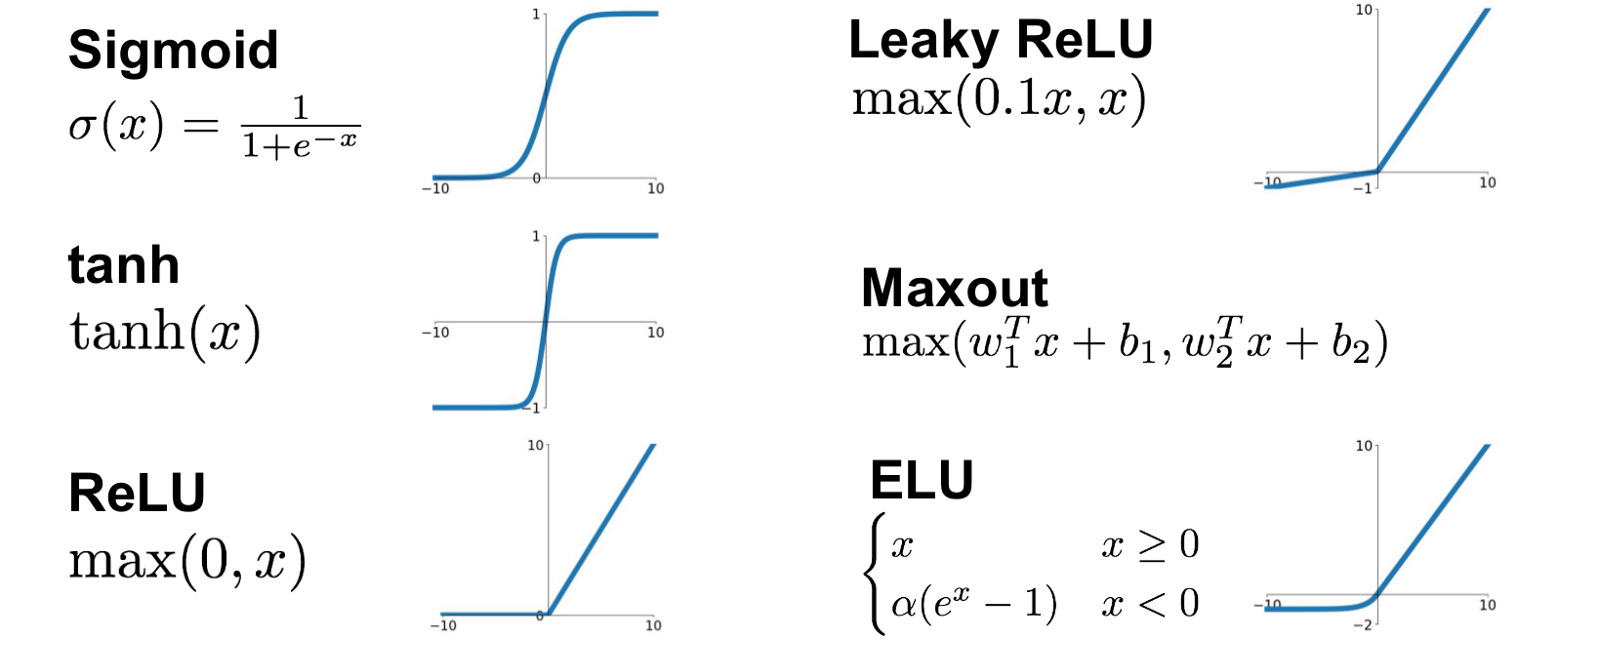
\includegraphics[width=\textwidth]{img/activation.png}
        \caption{Различные функции активации}
        \end{figure}
\end{frame}


\begin{frame}
    \frametitle{Функция потерь (Loss Function)}
    Чтобы обучать сеть, нам нужна мера того, насколько она ошибается в предсказании. Эту меру называют функцией потерь $L(\hat{y}, y)$, где:
    \begin{itemize}
        \item $\hat{y}$ --- предсказание сети.
        \item $y$ --- истинное значение.
    \end{itemize}
    \pause
    \textbf{Примеры:}
    \begin{itemize}
        \item \textbf{Для регрессии}: Среднеквадратичная ошибка (MSE)
        \[L_{MSE} = \frac{1}{m} \sum_{i=1}^{m} (\hat{y}^{(i)} - y^{(i)})^2 \]
        
        \item \textbf{Для бинарной классификации}: Бинарная кросс-энтропия
        \[L_{BCE} = -\frac{1}{m} \sum_{i=1}^{m} [y^{(i)}\log(\hat{y}^{(i)}) + (1-y^{(i)})\log(1-\hat{y}^{(i)})] \]
    \end{itemize}
\end{frame}


\begin{frame}
    \frametitle{Градиентный спуск}
    Наша цель --- найти такие параметры сети (веса $W$ и смещения $b$), которые минимизируют функцию потерь $L$.
    \vfill
    \begin{itemize}
        \item \textbf{Идея}: двигаться в направлении, противоположном градиенту функции потерь (т.е. в сторону наискорейшего убывания).
        \item \textbf{Градиент} $\nabla L$ --- это вектор частных производных $L$ по всем параметрам сети.
    \end{itemize}
    \vfill
    \begin{block}
    \centering
    Правило обновления весов для одного параметра $w$:
    \[ w := w - \eta \frac{\partial L}{\partial w} \]
    где $\eta$ --- \textbf{скорость обучения} (learning rate).
    \end{block}
\end{frame}


\begin{frame}
    \frametitle{Backpropagation}
    Как эффективно посчитать производную $\frac{\partial L}{\partial w}$ для веса, который находится в глубоком слое сети?
    \vfill
    \textbf{Метод обратного распространения ошибки (Backpropagation)} --- это, по сути, рекурсивное применение \textbf{цепного правила} (chain rule) из матанализа для вычисления градиентов.
    \vfill
    \begin{block}{Идея}
        \begin{enumerate}
            \item Сначала вычисляется производная ошибки по выходу последнего слоя.
            \item Затем эта ошибка движется назад, от слоя к слою.
            \item На каждом слое вычисляется градиент по его параметрам и градиент по его входу, который передается дальше назад.
        \end{enumerate}
    \end{block}
\end{frame}

\begin{frame}{Однослойный случай: градиент для одного нейрона}
  Пусть $L=\tfrac12(\hat y - y)^2$, $\hat y = \sigma(\bm{w}^\top \bm{x}+b)$.
  \[
    \frac{\partial L}{\partial \bm{w}} = \frac{\partial L}{\partial \hat y}\,\frac{d\hat y}{dz}\,\frac{\partial z}{\partial \bm{w}}
    = (\hat y - y)\,\sigma'(z)\,\bm{x}.
  \]
  Аналогично:
  \[
    \frac{\partial L}{\partial b} = (\hat y - y)\,\sigma'(z).
  \]
\end{frame}
\begin{frame}
    \frametitle{Многослойный случай}
    Рассмотрим производную потерь $L$ по весу $w_{ij}^{[l]}$ в слое $l$.
    \[ \frac{\partial L}{\partial w_{ij}^{[l]}} = \frac{\partial L}{\partial a^{[L]}} \frac{\partial a^{[L]}}{\partial z^{[L]}} \cdots \frac{\partial z^{[l+1]}}{\partial a^{[l]}} \frac{\partial a^{[l]}}{\partial z^{[l]}} \frac{\partial z^{[l]}}{\partial w_{ij}^{[l]}} \]
    
    Это выглядит сложно, но на практике вычисляется последовательно:
    \begin{enumerate}
        \item \textbf{Forward Pass}: Вычисляем все активации $a^{[l]}$ до самого конца.
        \item \textbf{Backward Pass}:
            \begin{itemize}
                \item Вычисляем градиент для последнего слоя $\frac{\partial L}{\partial z^{[L]}}$.
                \item Рекурсивно вычисляем $\frac{\partial L}{\partial z^{[l]}}$ через $\frac{\partial L}{\partial z^{[l+1]}}$.
                \item Используя $\frac{\partial L}{\partial z^{[l]}}$, находим градиенты по параметрам этого слоя: $\frac{\partial L}{\partial W^{[l]}}$ и $\frac{\partial L}{\partial b^{[l]}}$.
            \end{itemize}
    \end{enumerate}
\end{frame}
\begin{frame}{Инициализация весов}
Значимую роль играет начальная инициализация весов сети.
  \begin{itemize}
    \item Плохая инициализация → затухание/взрыв градиентов.
    \item Эвристический подход: случайные числа.
    \item Классические схемы: \textbf{Xavier/Glorot} (для tanh): распределение с дисперсией $\sim\frac{2}{n_{in}+n_{out}}$.
    \item \textbf{Kaiming He} (для ReLU): дисперсия $\sim\frac{2}{n_{in}}$.
  \end{itemize}
\end{frame}

\begin{frame}{Регуляризация}
  \begin{itemize}
    \item $L_2$ (или $L_1$) весовая регуляризация: добавить $\frac{\lambda}{2}\sum_\ell \|W^{(\ell)}\|_F^2$ в цель → дополнительный член $\lambda W^{(\ell)}$ в градиенте.
    \item Dropout (случайное зануление нейронов на обучении) и Batch normalization (контроль над средним и дисперсией).
    \item Ранняя останова (early stopping) по валидационной выборке.
  \end{itemize}
  
    \centering
          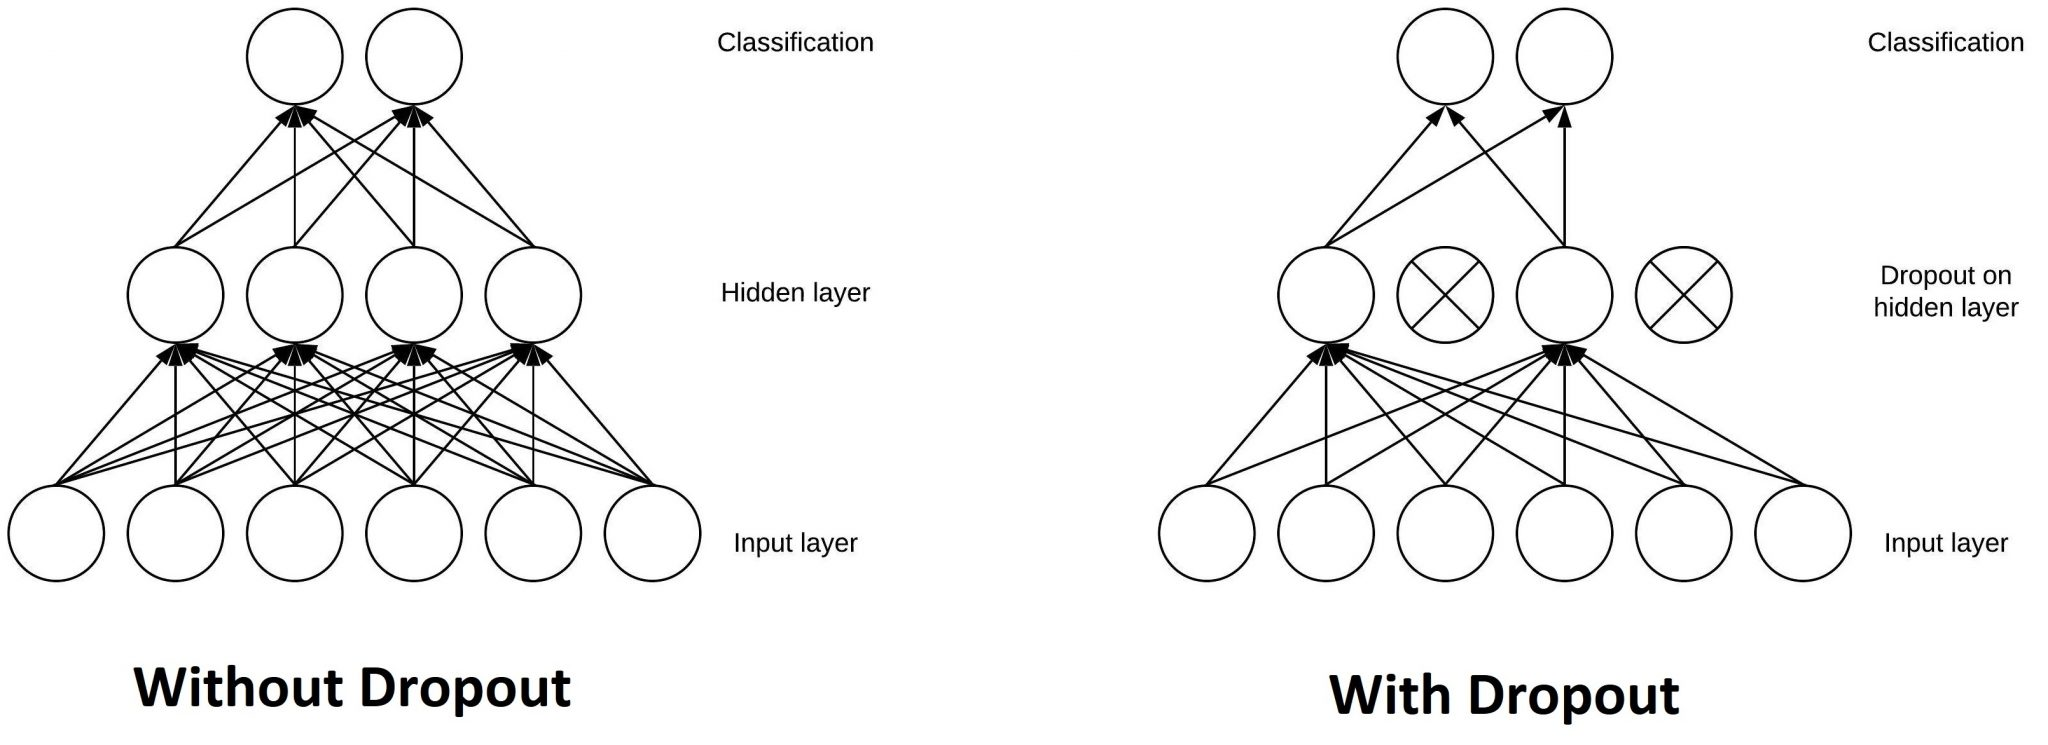
\includegraphics[width=0.8\textwidth]{img/dropout.png}
\end{frame}

\begin{frame}{Оптимизаторы стохастического спуска}
  \begin{itemize}
    \item SGD --- простой стохастический градиентный спуск.
    \item Моменты: $v\leftarrow \beta v + (1-\beta)\nabla_\theta J$, $\theta\leftarrow\theta-\eta v$.
    \item Адаптивные методы: AdaGrad, RMSProp, Adam.
  \end{itemize}
\end{frame}
\end{document}